\documentclass[tikz]{standalone}
\usepackage{pgfplots}
\pgfplotsset{compat=1.15}
\usepackage{mathrsfs}
\usetikzlibrary{arrows,calc}
\usepackage{tkz-euclide}
\pagestyle{empty}

\definecolor{AngleClr}{rgb}{0,0.39215686274509803,0}
\definecolor{ShapeClr}{rgb}{0.6,0.2,0}

\begin{document}

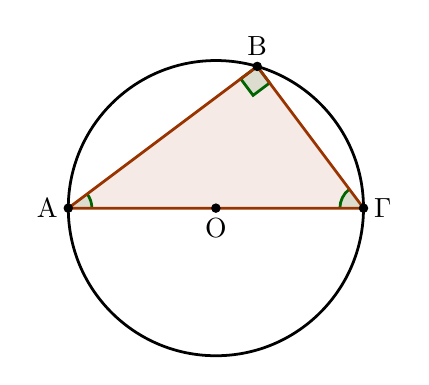
\begin{tikzpicture}[scale=.75]
\tkzSetUpLine[line width=1pt,color=black]
\tkzSetUpPoint[fill=black]

\tkzDefPoints{0/0/B,3.2/2.4/A,5/0/C,2.5/0/O}
\tkzDrawCircle[line width=1pt,color=black](O,A)

\tkzFillPolygon[fill=ShapeClr,fill opacity=0.1](A,B,C)
\tkzMarkRightAngle[line width=1pt, size=.35,color=AngleClr,fill=AngleClr,fill opacity=0.1](B,A,C)
\tkzFillAngles[fill=AngleClr,size=.4,fill opacity=0.1](C,B,A A,C,B)
\tkzMarkAngles[line width=1pt,size=.4,color=AngleClr](C,B,A A,C,B)

\tkzDrawPolygon[color=ShapeClr](A,B,C)
\tkzDrawPoints[size=3](A,B,C,O)
\tkzLabelPoint[above](A){$\rm B$}
\tkzLabelPoint[left](B){$\rm A$}
\tkzLabelPoint[right](C){$\rm \Gamma$}
\tkzLabelPoint[below](O){$\rm O$}


\end{tikzpicture}

\end{document}
